\section{The power family, Klein--Gordon and lower-order perturbations}
\label{power:sec}

This section (i) puts softening ``Duffing continua'', the focusing
Klein--Gordon ($\phi^4$) equation and MEMS touchdown into one family
$\partial_t^2u-\Delta u=F_p(u)$, $p\notin[-1,1]$, and proves the spectral
theorem for its ODE blowup in all angular sectors (a detailed version of
\cref{fw:thm-spec}, including the integer, logarithmic and Jordan cases);
(ii) compares it with the published results; (iii) treats damping and
restoring forces $\gamma\partial_tu+m^2u$, which destroy exact self-similarity,
via an ``asymptotically autonomous'' lemma (\cref{power:lem-lower-order}) that
the model sections can cite. Labels: \textbf{(K)} known (with reference),
\textbf{(P)} proved here, \textbf{(S)} sketched here, \textbf{(N)} numerical or
conjectural. Symbolic claims are checked in \texttt{code/power\_symbolic.py},
numerical ones in \texttt{code/power\_spectrum.py}.

\subsection{Industrial models and the unified family}
\label{power:subsec-models}

\paragraph{Duffing continua.} A string ($d=1$) or membrane ($d=2$) with density
$\varrho$, tension $\mathcal T$, viscous damping $c_v$, on a nonlinear Winkler
foundation with restoring force $k_1u-k_3u^3$ per unit area obeys
\begin{equation}\label{power:eq-duffing}
  \varrho\,\partial_t^2u+c_v\,\partial_tu-\mathcal T\Delta u+k_1u=k_3u^3 .
\end{equation}
For a \emph{softening} foundation ($k_3>0$; continuum version of the softening
Duffing oscillator \cite{NayfehMook1979,KovacicBrennan2011}) the potential
$\frac12k_1u^2-\frac14k_3u^4$ has a barrier at $u_b=(k_1/k_3)^{1/2}$, and
homogeneous motions above it escape in finite time. With $t=t_*t'$,
$x=(\mathcal T/\varrho)^{1/2}t_*x'$, $u=(\varrho/(k_3t_*^2))^{1/2}u'$ (primes dropped),
\begin{equation}\label{power:eq-nlkg}
  \partial_t^2u+\gamma\,\partial_tu+m^2u-\Delta u=u^3,\qquad
  \gamma=c_vt_*/\varrho,\quad m^2=k_1t_*^2/\varrho .
\end{equation}
Taking $t_*$ equal to the blowup time shows that $\gamma$, $m$ measure the
damping time and foundation period \emph{relative to the blowup time}. For
$\gamma=0$ this is the focusing cubic Klein--Gordon ($\phi^4$) equation.
Physical caveats: the cubic law is a truncation, so ``blowup'' means dynamic
escape (snap-through) and the self-similar profile describes the escaping
region only while the foundation law is valid; Euler--Bernoulli beams
($\partial_x^4$ instead of $-\Delta$) are not covered.

\paragraph{The unified family.} For $p\in\mathbb R\setminus[-1,1]$ let
\begin{equation}\label{power:eq-family}
  \partial_t^2u-\Delta u=F_p(u):=\operatorname{sgn}(p-1)\,|u|^{p-1}u,\qquad
  s:=\tfrac{2}{p-1}\in(-1,0)\cup(0,\infty).
\end{equation}
For $p>1$ this is the focusing power equation; for $p=-q<-1$ and $u=w>0$ it is
the MEMS equation $\partial_t^2w-\Delta w=-w^{-q}$ for the gap $w$ ($\lambda$ in
$-\lambda w^{-q}$ scales out), with $s=-\sigma=-\frac{2}{q+1}$ as in
\cref{mems:sec}. The sign makes the force point \emph{towards} the singularity
($u\to\infty$, resp.\ $w\to0$). The critical Sobolev exponent is
$s_c=\frac d2-s$. See \cref{power:tab-models}.

\begin{table}[ht]
\centering\small
\begin{tabular}{@{}lcccc@{}}
\toprule
model & $p$ & $s$ & $V_0=(s+1)(s+2)$ & $\omega_0=\min\{1,2s+2\}$\\
\midrule
softening string/membrane, $\phi^4$ & $3$ & $1$ & $6$ & $1$\\
focusing NLKG/NLW & $p>1$ & $\frac{2}{p-1}$ & $\frac{2p(p+1)}{(p-1)^2}$ & $1$\\
MEMS, general & $-q<-1$ & $-\frac{2}{q+1}$ & $\frac{2q(q-1)}{(q+1)^2}$ & $\min\{1,\frac{2(q-1)}{q+1}\}$\\
MEMS, parallel plate & $-2$ & $-\frac23$ & $\frac49$ & $\frac23$\\
\bottomrule
\end{tabular}
\caption{The unified family \eqref{power:eq-family}; $\omega_0$ is the spectral
gap of \cref{power:cor-gap}.}
\label{power:tab-models}
\end{table}

\subsection{ODE blowup and the excluded range \texorpdfstring{$-1\le p\le1$}{-1<=p<=1}}
\label{power:subsec-ode}

\begin{proposition}[ODE profile; \textbf{(P)}]\label{power:prop-ode}
Let $p\neq\pm1$, $s=\frac2{p-1}$. Then $u''=F_p(u)$ has a solution
$u_T=\kappa(T-t)^{-s}$, $\kappa>0$, iff $p\notin[-1,1]$, and then
\[
  \kappa^{p-1}=\operatorname{sgn}(p-1)\,s(s+1)=|s(s+1)|,\qquad
  V_0:=F_p'(u_T)(T-t)^2=p\,s(s+1)=(s+1)(s+2).
\]
For MEMS with general $\lambda$: $\kappa^{q+1}=\lambda/(\sigma(1-\sigma))$,
$V_0=\lambda q\kappa^{-q-1}=q\sigma(1-\sigma)=(1-\sigma)(2-\sigma)>0$ (note
$F'(w)=+\lambda qw^{-q-1}$).
\end{proposition}
\begin{proof}
$u_T''=s(s+1)\kappa(T-t)^{-s-2}$, $F_p(u_T)=\operatorname{sgn}(p-1)\kappa^p(T-t)^{-sp}$
and $sp=s+2$. For $s>0$ and $s\in(-1,0)$ the product $\operatorname{sgn}(p-1)s(s+1)$
is positive; for $p\in(-1,1)$, $s<-1$ and it is negative. Euler's relation
$uF_p'(u)=pF_p(u)$ gives $V_0=p\,s(s+1)$, and $ps=s+2$.
\end{proof}

\begin{remark}[Why $-1\le p\le1$ is excluded; \textbf{(P)}]\label{power:rem-small-p}
For $p\in(-1,1)$ a self-similar solution would have $s<-1$, so $u_T$
\emph{and} $\partial_tu_T$ tend to $0$: no singularity of $(u,\partial_tu)$; even
with the opposite sign (where $\kappa$ exists) it is non-generic, the
second eigenvalue family below starting at $-2s-2>0$. For the MEMS sign and
$0<q<1$ the gap closes with finite speed, $w\approx\sqrt{2E}(T-t)$, and for $q=1$
with a logarithmic correction, $w\approx(T-t)\sqrt{2|\log(T-t)|}$ (from
$\frac12w'^2+\log w=E$). Self-similar ODE blowup thus exists exactly for
$s\in(-1,0)\cup(0,\infty)$, which is also where $\omega_0>0$.
\end{remark}

\paragraph{Symmetries.} Besides $T$, the boosted profiles \eqref{fw:boost}
$u_{T,a}=\kappa(1-|a|^2)^{s/2}(T-t+a\cdot x)^{-s}$, $|a|<1$, blow up on the
spacelike hyperplane $\{t=T+a\cdot x\}$ and are stationary in similarity
variables, $\psi_a(\xi)=\kappa(1-|a|^2)^{s/2}(1+a\cdot\xi)^{-s}$; this holds verbatim
in the MEMS range. Space translations act trivially on $u_T$.

\subsection{The linearised operator and the free flow}
\label{power:subsec-linear}

With $\Psi=\Psi_*+\Phi$, $\Psi_*=(\kappa,s\kappa)$ in \eqref{fw:system},
$\partial_\tau\Phi=\mathbf L\Phi+\mathbf N(\Phi)$ on
$\mathcal H^k=H^k(B^d)\times H^{k-1}(B^d)$, where
\[
  \mathbf L\Phi=\begin{pmatrix}-\Lambda\phi_1-s\phi_1+\phi_2\\ \Delta\phi_1-\Lambda\phi_2-(s+1)\phi_2+V_0\phi_1\end{pmatrix},\quad
  \mathbf N(\Phi)=\begin{pmatrix}0\\ F_p(\kappa+\phi_1)-F_p(\kappa)-V_0\phi_1\end{pmatrix}.
\]
Since $\kappa>0$, $F_p$ is real analytic near $\kappa$ for every real $p$
(non-integer $p$ and the singular MEMS force included); for $k>\frac d2$ and
$\|\phi_1\|_{L^\infty}\le\kappa/2$, $\mathbf N$ is locally Lipschitz with a
quadratic bound. No regularity restriction on $p$ arises.

\begin{lemma}[Polynomial invariance; \textbf{(P)}]\label{power:lem-poly}
Let $\mathcal P_N$ be the polynomials of degree $\le N$ in $\xi$. Then $\mathbf L$
maps $\mathcal P_N^2$ into itself and acts on homogeneous parts of degree $j$
(modulo $\mathcal P_{j-1}^2$) as
$M_j=\bigl(\begin{smallmatrix}-s-j&1\\ V_0&-s-1-j\end{smallmatrix}\bigr)$, with
eigenvalues $1-j$ and $-2s-2-j$. For $V_0=0$ (the free operator $\mathbf L_0$)
they are $-s-j$, $-s-1-j$; in particular $\mathbf L_0(1,0)=-s(1,0)$. On
constants $\mathbf L$ has the eigenvalues $1$ (time translation) and $-2s-2$.
\end{lemma}
\begin{proof}
$\Lambda$ multiplies homogeneous polynomials of degree $j$ by $j$, $\Delta$
lowers the degree by two, and $\det(M_j-\mu)=(\mu+j-1)(\mu+j+2s+2)$ since
$V_0=(s+1)(s+2)$.
\end{proof}

So every eigenvalue of \cref{power:thm-spectrum} with a polynomial
eigenfunction is visible algebraically; the content of the theorem is that
there are no others. Note also that polynomial (collocation, Galerkin)
discretisations of $\mathbf L$ are \emph{exact} on $\mathcal P_N^2$ and cannot detect
non-polynomial eigenfunctions (\cref{power:subsec-numerics}).

\begin{lemma}[Free flow; (a) \textbf{(P)}, (b) \textbf{(S)}]\label{power:lem-free}
Let $\omega_k:=k-s_c=k-\frac d2+s$. (a) $-s$ is an eigenvalue of $\mathbf L_0$ on
every $\mathcal H^k$ (eigenfunction $(1,0)$, i.e.\ $u\equiv$ const), so the growth
bound of $e^{\tau\mathbf L_0}$ is $\ge-s$; in the MEMS range $-s=\sigma>0$ and the
free flow grows. (b) $\mathbf L_0=\tilde{\mathbf L}_0+\mathbf K$ with $\mathbf K$ of finite
rank and $\|e^{\tau\tilde{\mathbf L}_0}\|\le Me^{-\omega_k\tau}$. Hence, if $\omega_k>0$,
$\sigma(\mathbf L)\cap\{\operatorname{Re}\lambda>-\omega_k\}$ consists of isolated
eigenvalues of finite algebraic multiplicity.
\end{lemma}
\begin{proof}[Proof of (b), sketch]
For $|\beta|=k-1$ let $f=\partial^\beta\phi_1$, $g=\partial^\beta\phi_2$. Since
$\partial^\beta\Lambda=(\Lambda+k-1)\partial^\beta$, the free flow gives
$\partial_\tau f=-(\Lambda+s+k-1)f+g$, $\partial_\tau g=\Delta f-(\Lambda+s+k)g$, and
with $\int_B h\Lambda h=-\frac d2\int_Bh^2+\frac12\int_{\partial B}h^2$,
\begin{multline*}
  \tfrac12\tfrac{d}{d\tau}\bigl(\|\nabla f\|^2+\|g\|^2\bigr)
  =-\omega_k\bigl(\|\nabla f\|^2+\|g\|^2\bigr)\\
  -\tfrac12\int_{\partial B}\bigl(|\nabla f|^2-(\partial_rf)^2+(\partial_rf-g)^2\bigr)
  \le-\omega_k\bigl(\|\nabla f\|^2+\|g\|^2\bigr),
\end{multline*}
the boundary term having a sign because $\partial B$ is the light cone. So the
seminorm
\[
  E_k(\Phi)=\textstyle\sum_{|\beta|=k-1}\bigl(\|\nabla\partial^\beta\phi_1\|^2+\|\partial^\beta\phi_2\|^2\bigr)
\]
decays at rate $2\omega_k$. Its kernel $\mathcal P_{k-1}\times\mathcal P_{k-2}$ is
finite-dimensional and $\mathbf L_0$-invariant (\cref{power:lem-poly}), and
$E_k^{1/2}$ is equivalent to the quotient norm (Bramble--Hilbert), so $\mathbf L_0$
is block-triangular with a quotient block of growth bound $\le-\omega_k$ and a
finite-rank remainder. $\mathbf L'=(0,V_0\phi_1)$ is compact, and the rest is
\cite[Ch.~IV]{EngelNagel2000}. Rigorous inner products of this type are
constructed in \cite{Ostermann2024,Glogic2025}.
\end{proof}

\begin{remark}[Regularity threshold; the Lumer--Phillips step]\label{power:rem-LP}
The free decay rate is $\omega_k=k-s_c$, so exponential decay needs regularity
strictly above scaling, $k>s_c$; at $k=s_c$ one needs Strichartz estimates in
similarity coordinates \cite{Donninger2017,DonningerRao2018,Wallauch2022}. To
see the full gap one needs $k>s_c+\omega_0$; for MEMS $k>\frac d2+\sigma+\omega_0$
(e.g.\ $q=2$: $k\ge2$ for $d=1$, $k\ge3$ for $d=2$). The simplest
Lumer--Phillips argument, an inner product in which $\mathbf L_0$ itself is
dissipative with bound $-s$, is sharp by (a) and yields the rate
$\min\{1,s\}$; we believe this is the origin of the exponent $\min\{1,s_p\}$ in
\cite{Ostermann2024}. In the MEMS range it yields nothing ($-s=\sigma>0$; no
inner product makes $\mathbf L_0$ dissipative with negative bound), and the
splitting (b) is necessary. The finite-rank part is absorbed into the compact
perturbation, so the positive free eigenvalue $\sigma$ is harmless: it is not an
eigenvalue of $\mathbf L$.
\end{remark}

\subsection{The spectral theorem in all angular sectors}
\label{power:subsec-spectrum}

Let $\mathcal Y_\ell$ be the spherical harmonics of degree $\ell$ ($d\ge2$); for
$d=1$, $\mathcal Y_0=\{1\}$, $\mathcal Y_1=\{\operatorname{sgn}\xi\}$, $\mathcal Y_{\ell\ge2}=\{0\}$.

\begin{theorem}[Spectrum of the ODE blowup; \textbf{(P)}]\label{power:thm-spectrum}
Let $d\ge1$, $p\in\mathbb R\setminus[-1,1]$, $k\in\mathbb N$, $\omega_k>0$, and
$\operatorname{Re}\lambda>-\omega_k$. Then $\lambda$ is an eigenvalue of $\mathbf L$ on
$\mathcal H^k$ iff
\[
  \lambda\in\Sigma_s:=\{1-\ell-2n\}\cup\{-2s-2-\ell-2n\},\qquad n\in\mathbb N_0,\ \mathcal Y_\ell\neq\{0\}.
\]
In the sector $\ell$ the eigenfunctions are $(g,(\lambda+s+\Lambda)g)$,
$g=|\xi|^\ell Y_\ell\,{}_2F_1(\alpha,\beta;\frac d2+\ell;|\xi|^2)$, $Y_\ell\in\mathcal Y_\ell$,
$\alpha=\frac{\lambda+\ell-1}{2}$, $\beta=\frac{\lambda+\ell+2s+2}{2}$ (a polynomial of
degree $n$ in $|\xi|^2$). All eigenvalues are real, and:
\begin{enumerate}[nosep,label=(\alph*)]
\item $\lambda=1$ occurs only for $\ell=0$, with $\Phi=(1,s+1)=$ time-translation mode;
\item $\lambda=0$ occurs only for $\ell=1$, with $\Phi=(\xi_j,(s+1)\xi_j)$,
  $j=1,\dots,d$, the boost modes $\propto\partial_{a_j}\Psi_a|_{a=0}$;
\item both are semisimple. The two families collide iff $s\in\frac12+\mathbb Z$
  ($p\in\{5,\frac73,\frac95,\dots\}$ or $q=3$); at the lowest collisions
  ($s=-\frac12,\lambda=-1$; $s=\frac12,\lambda=-3$; $\ell=0$) there is a Jordan block of
  length two.
\end{enumerate}
\end{theorem}

\begin{proof}
\emph{Reduction.} An eigenfunction has $\phi_2=(\lambda+s+\Lambda)\phi_1$, and
$g=\phi_1$ solves \eqref{fw:eig} with $a=s+\lambda$, which is elliptic in the open
ball; so $g\in C^\infty(B^d)$. Each spherical-harmonic component
$|\xi|^\ell Y_\ell h(|\xi|^2)$ is again an $H^k$ solution, and $h$ solves
\eqref{fw:hyp} with $c=\frac d2+\ell$, $\alpha+\beta+1=a+\ell+\frac32$,
$\alpha\beta=\frac14[(a+\ell)(a+\ell+1)-V_0]$; with $a_1=s+1$, $a_2=-(s+2)$ this
gives the stated $\alpha,\beta$. (The sector $\ell$ in dimension $d$ is the radial
problem in dimension $d+2\ell$ with $\lambda\mapsto\lambda+\ell$.)
\emph{At $z=0$} the second Frobenius solution gives $|\xi|^{2-d-\ell}Y_\ell$ (or
$\log|\xi|$, or $|\xi|$, $\operatorname{sgn}\xi$ for $d\le2$), which is not smooth; so
$h\propto{}_2F_1(\alpha,\beta;c;z)$.
\emph{At $z=1$} the exponents are $0$ and $\mu=\frac{d-1}{2}-s-\lambda$; the non-analytic
local solutions behave like $(1-|\xi|^2)^\mu$, $(1-|\xi|^2)^m\log(1-|\xi|^2)$ ($\mu=m\in\mathbb
N_0$) or $(1-|\xi|^2)^{-m}$ ($\mu=-m<0$), and lie in $H^k$ near $\partial B$ only if
$\operatorname{Re}\mu>k-\frac12$, i.e.\ $\operatorname{Re}\lambda<-\omega_k$. Hence, for
$\operatorname{Re}\lambda>-\omega_k$, $h$ is an eigenfunction iff it is analytic at $z=1$.
\emph{Monodromy.} The hypergeometric equation is Fuchsian with singular points
$0,1,\infty$. A solution analytic at $0$ and at $1$ has trivial monodromy and
extends to an entire function of polynomial growth (as $\infty$ is regular
singular), i.e.\ a polynomial; and ${}_2F_1(\alpha,\beta;c;z)$ is a polynomial iff
$\alpha\in-\mathbb N_0$ or $\beta\in-\mathbb N_0$. This handles the integer and logarithmic
cases uniformly (alternatively use the connection formulae
\cite[\S15.8]{OlverEtAl2010}). $\alpha=-n$ gives $\lambda=1-\ell-2n$, $\beta=-n$ gives
$\lambda=-2s-2-\ell-2n$.
\emph{(a), (b)}: $1-\ell-2n\ge0$ iff $(\ell,n)\in\{(0,0),(1,0)\}$, and
$-2s-2-\ell-2n<0$ for $s>-1$.
\emph{(c)}: a generalised eigenvector solves $(\mathbf L-\lambda)\Phi=\Phi_\lambda$;
eliminating $\phi_2$ gives an inhomogeneous hypergeometric equation with
polynomial right-hand side, so by the same monodromy argument an $\mathcal H^k$
solution is a polynomial. By \cref{power:lem-poly} its degree is at most
$\max\{\deg\Phi_\lambda,j_*\}$, where $M_{j_*}-\lambda$ is singular, and the
degree-$j_*$ block requires the top part of $\Phi_\lambda$ to lie in
$\operatorname{ran}(M_{j_*}-\lambda)$. For $\lambda=1$ ($j_*=0$) and $\lambda=0$ ($j_*=1$) this
fails, as $\lambda$ is a simple eigenvalue of $M_{j_*}$ for $s>-1$. At a collision
both $\alpha,\beta\in-\mathbb N_0$ and the eigenfunction is shared by the two families
(e.g.\ $s=-\frac12$, $\lambda=-1$: $g\equiv1$), and a generalised eigenvector exists:
$(\mathbf L+1)\Phi=(1,-\frac32)$ with $\phi_1=-|\xi|^2/3$ ($d=3$), and for $s=\frac12$,
$\lambda=-3$, $(\mathbf L+3)\Phi=(1,-\frac52)$ with $\phi_1=-\frac23|\xi|^2+\frac2{15}|\xi|^4$ ($d=3$). That all non-colliding eigenvalues
are semisimple, and all collisions give Jordan blocks (a double zero of
$1/(\Gamma(\alpha)\Gamma(\beta))$), is expected but only checked in these cases
\textbf{(S)}.
\end{proof}

\begin{corollary}[Spectral gap; \textbf{(P)}]\label{power:cor-gap}
If $\omega_k>\omega_0$, then
$\sup\{\operatorname{Re}\lambda:\lambda\in\sigma(\mathbf L)\setminus\{0,1\}\}=-\omega_0$,
\[
  \omega_0=\min\{1,2s+2\}=\begin{cases}1,& p>1\text{ or }p=-q,\ q\ge3,\\[2pt]
  \frac{2(q-1)}{q+1},& p=-q,\ 1<q\le3.\end{cases}
\]
The gap eigenvalue is $-1$ ($\ell=0,n=1$ and $\ell=2,n=0$) for $p>1$, $q\ge3$, and
the spatially homogeneous mode $-2s-2=-2(1-\sigma)$ for $q<3$; at $q=3$ they form a
Jordan block. For the parallel-plate force $q=2$: $\omega_0=\frac23$.
\end{corollary}

\subsection{What is proved in the literature}
\label{power:subsec-lit}

All results below concern $p>1$; for the MEMS range see \cref{mems:sec}.
\textbf{(K)}:
% TODO verify: range 1<p<=3 in DS2012; data space/range in DS2017; rate in Ostermann Thm 1.1;
% content of MerleZaag2016 (full texts not accessed, see "Source check" below)
\cite{DonningerSchoerkhuber2012}: $d=3$, radial, $1<p\le3$, stability of $u_T$ in
the energy topology (complementing \cite{MerleZaag2003,MerleZaag2007}); here
$k=1$ and $\omega_1=s-\frac12\ge\frac12$, consistent with \cref{power:rem-LP}.
\cite{DonningerSchoerkhuber2014}: $d=3$, radial, $p>3$, an open set of radial data
above energy regularity blows up via $u_T$.
\cite{DonningerSchoerkhuber2016}: $d=3$, energy supercritical, \emph{no symmetry
assumption}. \cite{DonningerSchoerkhuber2017}: radial data in odd $d\ge5$,
energy-supercritical powers, data in $H^{(d+1)/2}\times H^{(d-1)/2}$.
\cite{Ostermann2024}: all $d\ge1$, all $p>1$, no symmetry; data in
$H^k\times H^{k-1}$, $k>\frac d2$; convergence to a Lorentz-boosted ODE profile with
parameters $(T^*,\beta^*)$, with decay exponent governed by $\min\{1,s_p\}$;
dissipative inner products on $H^k$ for all $d$ and integer $k$.
\cite{Liu2025}: superconformal powers, all dimensions, mode stability via Lorentz
transformations and asymptotic stability of the ODE blowup family, extending
\cite{MerleZaag2016} (subconformal, energy space, explicit Lorentz family, no
symmetry) and \cite{Ostermann2024}. Critical case $d=3$, $p=5$:
\cite{Donninger2017,DonningerRao2018}; cubic in higher dimensions:
\cite{ChatzikaleasDonninger2019}.

\emph{Cross-check.} In all these works the only non-negative eigenvalues are
$\lambda=1$ and, nonradially, $\lambda=0$, as in \cref{power:thm-spectrum}. The
exponent $\min\{1,s_p\}$ of \cite{Ostermann2024} equals the gap $\omega_0=1$ for
$p\le3$ but is smaller for $p>3$; it reflects the free eigenvalue $-s$ of
constants (\cref{power:rem-LP}), not an eigenvalue of $\mathbf L$ (the second
family starts at $-2s-2<-s$). With \cref{power:lem-free}(b) the rate should
improve to $\min\{1,\omega_k\}-\varepsilon$, i.e.\ $1-\varepsilon$ for $k$ large
\textbf{(S)}. \emph{Source check:} the full texts could not be accessed here;
the statements are taken from abstracts/indexing data and
\texttt{bib/lit.bib}, and the details (ranges of $p$, spaces, rates) should be
checked against the papers.

\subsection{Lower-order perturbations: damping and restoring forces}
\label{power:subsec-lower}

Consider, with $\gamma,m^2\in\mathbb R$,
\begin{equation}\label{power:eq-pert}
  \partial_t^2u+\gamma\,\partial_tu+m^2u-\Delta u=F_p(u).
\end{equation}
With $T-t=Te^{-\tau}$ and \eqref{fw:psi} one obtains \emph{exactly}
(\textbf{(P)}, symbolic identity)
\begin{equation}\label{power:eq-sim-pert}
  \partial_\tau\Psi=\mathbf L_0\Psi+\begin{pmatrix}0\\F_p(\psi_1)\end{pmatrix}
  -\begin{pmatrix}0\\ \gamma Te^{-\tau}\psi_2+m^2T^2e^{-2\tau}\psi_1\end{pmatrix}:
\end{equation}
non-autonomous terms of size $e^{-\tau}$ (damping) and $e^{-2\tau}$ (mass), with $T$
in the coefficients.

\begin{proposition}[Perturbed ODE blowup; expansion \textbf{(P)}, existence
\textbf{(S)}]\label{power:prop-ode-pert}
As $\rho=T-t\downarrow0$, spatially homogeneous solutions of \eqref{power:eq-pert}
blowing up at $T$ form a one-parameter family,
\begin{gather*}
  U_T=\kappa\rho^{-s}\bigl(1+a_1\rho+a_2\rho^2+\dots\bigr)+c\,\rho^{s+2}(1+\dots),\\
  a_1=\frac{\gamma s}{2(2s+1)},\qquad
  a_2=\frac{\gamma^2(3s^2-5s-4)}{24(2s+1)^2}+\frac{m^2}{6s}.
\end{gather*}
The order-$j$ coefficient obeys $-(j+1)(2s+2-j)a_j=$ (lower orders); the indicial
roots $j=-1$, $j=2s+2$ are the eigenvalues $1$, $-2s-2$ of \cref{power:lem-poly}. If
$2s+2\in\mathbb N$ and compatibility fails, $\rho^{2s+2}\log\rho$ terms appear: for
$p=3$ iff $\gamma^2(9m^2-2\gamma^2)\neq0$ (cf.\ the Painlevé condition $m^2=2\gamma^2/9$
for the damped Duffing equation), for $p=5$ iff $\gamma(16m^2-3\gamma^2)\neq0$, and
for MEMS $q=3$ at first order whenever $\gamma\ne0$:
$U_T=\sqrt2\rho^{1/2}(1+\frac\gamma4\rho\log\rho+c\rho+\dots)$. Hence
$\Psi_T(\tau)-\Psi_*=O(e^{-\tau})$ if $\gamma\neq0$ ($O(\tau e^{-\tau})$ for $q=3$) and
$O(e^{-2\tau})$ if $\gamma=0$.
\end{proposition}

\begin{lemma}[The tilted family survives damping; \textbf{(P)}]\label{power:lem-tilt}
For $|a|<1$, $u=W(T-t+a\cdot x)$ solves \eqref{power:eq-pert} iff
$(1-|a|^2)W''-\gamma W'+m^2W=F_p(W)$. Hence
$u_{T,a}(t,x):=U^{\gamma_a}\bigl((T-t+a\cdot x)/\sqrt{1-|a|^2}\bigr)$, with $U^{\gamma_a}(\rho)$ the
perturbed ODE blowup of \cref{power:prop-ode-pert} for damping
$\gamma_a=\gamma/\sqrt{1-|a|^2}$, is an exact solution blowing up on
$\{t=T+a\cdot x\}$, and $\Psi_{T,a}(\tau)=\Psi_a+O(e^{-\tau})$.
\end{lemma}
\begin{proof}
$\partial_t^2u=W''$, $\Delta u=|a|^2W''$, $\partial_tu=-W'$; then rescale the
argument of $W$ by $\sqrt{1-|a|^2}$.
\end{proof}

Thus the mass preserves Lorentz invariance (for $\gamma=0$ the $u_{T,a}$ are
boosts of $U_T$) and damping breaks it, but the $d$-parameter tilted family
remains an exact family of solutions for every $\gamma$; only translation
invariance in $(t,x)$ is used. The neutral modes $\lambda=0$ are therefore still
generated by exact solutions, and no dynamical modulation of the boost
parameter (as anticipated in \cref{fw:subsec-lower}) is needed.

\begin{lemma}[Asymptotically autonomous Lyapunov--Perron lemma; \textbf{(S)}]
\label{power:lem-lower-order}
Let $\mathbf L$ generate a $C_0$-semigroup $\mathbf S$ on a Hilbert space $\mathcal H$,
$\mathbf P=\mathbf P_1+\mathbf P_0$ a finite-rank projection commuting with $\mathbf S$,
$\mathbf L\mathbf P_1=\mathbf P_1$, $\mathbf L\mathbf P_0=0$, and
$\|\mathbf S(\tau)(\mathbf I-\mathbf P)\|\le Me^{-\bar\omega\tau}$ for some $\bar\omega\in(0,1]$. For
$\theta$ in a closed ball $\overline B\subset\mathbb R^{\operatorname{rank}\mathbf P}$ let
$\mathbf B_\theta(\tau)\in\mathcal B(\mathcal H)$ be strongly continuous with
$\sup_\tau\|\mathbf B_\theta(\tau)\|\le\beta$ (in applications
$\mathbf B_\theta(\tau)=O(|a|)+O(e^{-\tau})$), and $\mathbf N_\theta(\tau,\cdot)$ with
$\mathbf N_\theta(\tau,0)=0$,
$\|\mathbf N_\theta(\tau,\Phi)-\mathbf N_\theta(\tau,\tilde\Phi)\|\le C_N(\|\Phi\|+\|\tilde\Phi\|)\|\Phi-\tilde\Phi\|$
for $\|\Phi\|,\|\tilde\Phi\|\le1$, all continuous in $\theta$. Consider
\begin{equation}\label{power:eq-abstract}
  \partial_\tau\Phi=\mathbf L\Phi+\mathbf B_\theta(\tau)\Phi+\mathbf N_\theta(\tau,\Phi),\qquad\Phi(0)=\mathbf u_\theta .
\end{equation}
For every $\omega\in(0,\bar\omega)$ there are $\beta_0,\delta_0,C>0$ such that if $\beta\le\beta_0$ and
$\|\mathbf u_\theta\|\le\delta\le\delta_0$:
\begin{enumerate}[nosep,label=(\roman*)]
\item there is a unique $\Phi_\theta$ with $\sup_\tau e^{\omega\tau}\|\Phi_\theta(\tau)\|\le
  C\delta$ solving
  $\Phi(\tau)=\mathbf S(\tau)[\mathbf u_\theta-\mathbf C_\theta(\Phi)]+\int_0^\tau\mathbf S(\tau-\sigma)\mathbf G_\theta(\sigma)\,d\sigma$,
  where $\mathbf G_\theta=\mathbf B_\theta\Phi+\mathbf N_\theta(\sigma,\Phi)$ and
  $\mathbf C_\theta(\Phi)=\mathbf P\mathbf u_\theta+\int_0^\infty(e^{-\sigma}\mathbf P_1+\mathbf P_0)\mathbf G_\theta(\sigma)\,d\sigma$;
\item $\Phi_\theta$ solves \eqref{power:eq-abstract} iff $\mathbf C_\theta(\Phi_\theta)=0$;
\item if $\theta\mapsto\mathbf P\mathbf u_\theta$ is a homeomorphism onto a neighbourhood of
  $0$ in $\operatorname{ran}\mathbf P$ with $\delta$-independent Lipschitz inverse
  (transversality), then for small $\delta$ some $\theta^*$ has
  $\mathbf C_{\theta^*}(\Phi_{\theta^*})=0$.
\end{enumerate}
An inhomogeneity $e^{-\tau}\mathbf g_\theta(\tau)$, $\|\mathbf g_\theta\|\le\delta$, may be
added; then (i)--(iii) hold for $\omega<\min\{\bar\omega,1\}$.
\end{lemma}
\begin{proof}[Sketch]
In $\mathcal X=\{\Phi:\|\Phi\|_{\mathcal X}=\sup e^{\omega\tau}\|\Phi(\tau)\|<\infty\}$,
\[
  \int_0^\tau\!Me^{-\bar\omega(\tau-\sigma)}\bigl(\beta e^{-\omega\sigma}\|\Phi\|_{\mathcal X}
  +C_Ne^{-2\omega\sigma}\|\Phi\|_{\mathcal X}^2\bigr)d\sigma
  \le Me^{-\omega\tau}\Bigl(\tfrac{\beta}{\bar\omega-\omega}\|\Phi\|_{\mathcal X}+\tfrac{C_N}{\omega}\|\Phi\|_{\mathcal X}^2\Bigr),
\]
while the corrected unstable and neutral parts
$-\int_\tau^\infty(e^{\tau-\sigma}\mathbf P_1+\mathbf P_0)\mathbf G_\theta\,d\sigma$ are
$O(\beta\omega^{-1}e^{-\omega\tau}\|\Phi\|_{\mathcal X}+C_Ne^{-2\omega\tau}\|\Phi\|_{\mathcal X}^2)$. So the map is
a contraction on a small ball if $\beta\le\beta_0$; a decay factor $e^{-\sigma}$ in
$\mathbf B_\theta$ makes the term integrable but not small, which is why the
smallness of $\beta$ (\cref{power:rem-small-beta}) is needed. A forcing is handled
by $\int_0^\tau e^{-\bar\omega(\tau-\sigma)}e^{-\sigma}d\sigma\le(1+\tau)e^{-\min\{\bar\omega,1\}\tau}$.
(ii), (iii) are as in \cite{DonningerSchoerkhuber2012,Ostermann2024} (Brouwer).
\end{proof}

\begin{remark}[Making $\beta$ small]\label{power:rem-small-beta}
Linearising \eqref{power:eq-sim-pert} at the exact family $\Psi_{T,a}(\tau)$ of
\cref{power:lem-tilt} gives \eqref{power:eq-abstract} with $\theta=(T,a)$, no
inhomogeneity, and
$\mathbf B_\theta(\tau)\Phi=\bigl(0,[F_p'(\psi_{T,a,1}(\tau))-V_0]\phi_1-\gamma Te^{-\tau}\phi_2-m^2T^2e^{-2\tau}\phi_1\bigr)$,
so $\beta\lesssim|a|+|\gamma|T+m^2T^2$. Here $|a|=O(\delta)$; to make the rest small, evolve
the data to $t_1=1-\eta$ by local well-posedness on balls (finite speed of
propagation keeps the solution $C(\eta)\varepsilon$-close to the reference on
$B_{\eta+\delta}$) and rescale by $\eta$: $(\gamma,m^2)\mapsto(\gamma\eta,m^2\eta^2)$.
\end{remark}

\begin{theorem}[ODE blowup under lower-order terms; \textbf{(S)},
conditional]\label{power:thm-lower-order}
Let $d\ge1$, $p\in\mathbb R\setminus[-1,1]$, $\gamma,m^2\in\mathbb R$, $k\in\mathbb N$,
$k>\max\{\frac d2,s_c\}$, and let $\bar\omega\in(0,1]$ be such that the autonomous estimate
$\|\mathbf S(\tau)(\mathbf I-\mathbf P)\|_{\mathcal H^k}\lesssim e^{-\bar\omega\tau}$ holds (by
\cref{power:thm-spectrum,power:lem-free} any $\bar\omega<\min\{\omega_0,\omega_k\}$; for $p>1$
and $\bar\omega<\min\{1,s\}$ this is contained in \cite{Ostermann2024}, as we read
it), and $0<\omega<\bar\omega$. Let $U$ be a spatially homogeneous solution of \eqref{power:eq-pert} on
$[0,1)$ with ODE blowup at $1$. There is $\varepsilon>0$ such that for data with
$\|(u_0,u_1)-(U(0),U'(0))\|_{H^k\times H^{k-1}(B_{1+\varepsilon})}\le\varepsilon$ there exist
$T^*$ near $1$ and small $a^*\in\mathbb R^d$ ($a^*=0$ for radial data) such that
$u$ blows up at $(T^*,0)$ and
\[
  \|\Psi(\tau)-\Psi_{T^*,a^*}(\tau)\|_{\mathcal H^k}\lesssim e^{-\omega\tau},\qquad
  \|\Psi(\tau)-\Psi_{a^*}\|_{\mathcal H^k}\lesssim e^{-\omega\tau}+e^{-\tau}
\]
($e^{-2\tau}$ instead of $e^{-\tau}$ if $\gamma=0$; $\tau e^{-\tau}$ for $q=3$,
$\gamma\neq0$). The blowup point is not a modulation parameter: any $x_0$ near $0$
may replace $0$, and then $(T^*,a^*)$ depend on $x_0$ ($a^*$ is the slope of the
blowup surface for the exact tilted solutions, and presumably to leading order
in general).
\end{theorem}
\begin{proof}[Sketch]
Reduce to small $(\gamma,m^2)$ (\cref{power:rem-small-beta}); $\mathbf N_\theta$ is
quadratic uniformly in $\tau$ because $\psi_{T,a,1}(\tau)$ stays within $\kappa/4$ of
$\psi_a$. Transversality: by \cref{power:prop-ode-pert,power:lem-tilt},
$\partial_T\Psi_{T,a}(0)$ and $\partial_{a_j}\Psi_{T,a}(0)$ are, up to nonzero factors and
errors $O(|\gamma|+m^2+|a|)$, the eigenfunctions of
\cref{power:thm-spectrum}(a),(b). Apply \cref{power:lem-lower-order}; the second
estimate follows from \cref{power:lem-tilt}.
\end{proof}

\begin{remark}[Rates and resonances]\label{power:rem-rates}
(1) Since $\omega_0\le1$ in the whole family, damping and mass never decay
\emph{slower} than the gap. If one linearises at $\Psi_a$ instead of
$\Psi_{T,a}(\tau)$, the forcing has rate $1$ (damping) or $2$ (mass); for
$\omega_0=1$ rate-$1$ forcing can resonate with the eigenvalue $-1$ and produce
$\tau e^{-\tau}$ (for $a\neq0$ the forcing has $\ell=2$ components), and at $q=3$ the
Jordan block at $-1$ does the same. Only the exponent is affected.
(2) Lower-order nonlinear terms $f$ with $|f^{(j)}(u)|\lesssim|u|^{p'-j}$ contribute
$(T-t)^{s+2}f((T-t)^{-s}\psi_1)=O(e^{-s(p-p')\tau})$; they are perturbative iff
$s(p-p')>0$ ($p'<p$ for powers, weaker singularity $q'<q$ for MEMS; a constant
load has rate $s+2$). If $s(p-p')<\omega_0$ the convergence rate drops to
$s(p-p')$ but \cref{power:lem-lower-order} still applies; this is the only way
a perturbation in this family decays more slowly than the gap.
(3) The reduction, the tilted family and the abstract lemma are elementary;
the deep input is the autonomous linear estimate, the same as in
\cite{Ostermann2024}. Local well-posedness on balls for \eqref{power:eq-pert} and the
Lipschitz dependence on $\theta$ are routine and not written out.
\end{remark}

\paragraph{Literature on the perturbed equations \textbf{(K)}.}
% TODO verify the precise classes of perturbations in Hamza--Zaag and the statements in KSV14 / DW21
Hamza and Zaag constructed Lyapunov functionals in similarity variables for
$\partial_t^2u=\Delta u+|u|^{p-1}u+f(u)+g(\partial_tu)$ with lower-order $f,g$ (including
the Klein--Gordon mass and linear damping) and proved ODE-type blowup rates:
subconformal \cite{HamzaZaag2010}, conformal \cite{HamzaZaag2012}, Klein--Gordon
and other perturbations \cite{HamzaZaag2013}, superconformal
\cite{HamzaZaag2013b}. Killip, Stovall and Visan \cite{KillipStovallVisan2014}
obtained ODE-type blowup behaviour for focusing NLKG, so the mass is a
lower-order effect at blowup. The closest semigroup result we know is
\cite{DonningerWallauch2021} on strongly perturbed wave equations, where the
blowup solution is no longer self-similar; we could not check whether it covers
$\gamma\partial_tu$. To our knowledge (search not exhaustive) no Donninger-type
stability theorem for the damped NLW or NLKG has been published;
\cref{power:thm-lower-order} suggests that little beyond the autonomous theory
is needed.

\subsection{Non-ODE self-similar profiles}
\label{power:subsec-nontrivial}

In the energy-supercritical range there are self-similar solutions
$u=(T-t)^{-s}U(|x|/(T-t))$ with $U\not\equiv\kappa$. \textbf{(K)}; the explicit
formulas below were re-verified symbolically \textbf{(P)}.
% TODO verify: parity/range of p and mode count in BMW07; normalisation in GS21; dimensions in CGS24
\begin{itemize}[leftmargin=1.2em,nosep]
\item Bizoń--Maison--Wasserman \cite{BizonMaisonWasserman2007}: $d=3$, odd $p\ge7$,
  a countable family $U_n$ ($U_0=\kappa$); numerically $U_n$ has $n$ unstable modes
  besides time translation, and $U_1$ is conjectured to be the
  co-dimension-one critical solution between blowup and dispersal \textbf{(N)}.
\item Glogić--Schörkhuber \cite{GlogicSchoerkhuber2021}: cubic, explicit profile
  in every $d\ge5$, co-dimension-one stable without symmetry assumptions in
  $d=7$. One checks that ($\rho=|x|/(T-t)$)
  \[
    u^*=\frac{1}{T-t}\,\frac{2\sqrt2\sqrt{(d-1)(d-4)}}{d-4+3\rho^2}\quad\text{solves }\partial_t^2u-\Delta u=u^3
    \qquad\Bigl(d=7:\ u^*=\frac{4(T-t)}{(T-t)^2+|x|^2}\Bigr).
  \]
\item Csobo--Glogić--Schörkhuber \cite{CsoboGlogicSchoerkhuber2024}: quadratic,
  explicit profile for $d\ge7$, co-dimension-one stable in $d=9$; extended beyond
  the light cone in \cite{ChenEtAl2024}. One checks that in $d=9$
  \[
    u^*=\frac{1}{(T-t)^2}\,\frac{240\,(7-\rho^2)}{(7+5\rho^2)^2}\quad\text{solves }\partial_t^2u-\Delta u=u^2,
  \]
  and is positive in the cone; we expect, but have not confirmed, that this is
  their profile.
\end{itemize}
These live in high dimensions and are irrelevant for strings and membranes
($d\le2$), where the ODE profile is the generic one. MEMS profiles:
\cref{mems:sec}.

\subsection{Numerical confirmation}
\label{power:subsec-numerics}

By \cref{power:lem-poly}, Chebyshev collocation reproduces the polynomial
eigenvalues exactly and cannot see others; in double precision the lower ones
are also badly conditioned (spurious ``continuum'' for
$\operatorname{Re}\lambda<\frac{d-1}{2}-s$, where $(1-|\xi|^2)^\mu$ is continuous). We use
collocation ($N=24$, $V_0=F_p'(\kappa)$ computed numerically from $F_p$, so the
MEMS signs are tested) only for the well-conditioned eigenvalues $1,0,-1,-2s-2$,
and test completeness by a \emph{monodromy test} mirroring the proof: the
Frobenius solution regular at $z=0$ is continued numerically (DOP853, tolerance
$10^{-12}$) around $|z-1|=\frac12$; it returns to itself iff it is single-valued at
$z=1$, and single-valued solutions with a pole are rejected via their Laurent
coefficients. \Cref{power:tab-num} lists the zeros on a fine real grid ($d=3$):
all lie within $10^{-6}$ of $\Sigma_s$ and there are no others; on the complex box
$\operatorname{Re}\lambda\in[-4.5,1.3]$, $\operatorname{Im}\lambda\in[0.2,3]$ the defect stays
$\ge4\cdot10^{-4}$. At $q=3$ the defect vanishes quadratically at $\lambda=-1$
($10^{-4},10^{-6},10^{-8}$ at distances $10^{-2},10^{-3},10^{-4}$: Jordan block), at
$q=2$ linearly. \textbf{(N)}

\begin{table}[ht]
\centering\small
\begin{tabular}{@{}llll@{}}
\toprule
case ($d=3$) & $\ell=0$ & $\ell=1$ & $\ell=2$\\
\midrule
$p=3$ ($s=1$) & $1,-1,-3,-4$ & $0,-2,-4$ & $-1,-3$\\
$p=7$ ($s=\frac13$) & $1,-1,-\frac83,-3$ & $0,-2,-\frac{11}3,-4$ & $-1,-3$\\
$p=-2$ ($q=2$) & $1,-\frac23,-1,-\frac83,-3$ & $0,-\frac53,-2,-\frac{11}3,-4$ & $-1,-\frac83,-3$\\
$p=-3$ ($q=3$) & $1,-1^{(2)},-3^{(2)}$ & $0,-2^{(2)},-4^{(2)}$ & $-1,-3^{(2)}$\\
\bottomrule
\end{tabular}
\caption{Eigenvalues in $[-4.6,1.3]$ from the monodromy test; $^{(2)}$: collision
of the two families (double zero). The single-valued pole solution
${}_2F_1=(1-z)^{-1}$ at $p=3$, $\ell=2$, $\lambda=1$ is correctly rejected.}
\label{power:tab-num}
\end{table}

\begin{figure}[ht]
\centering
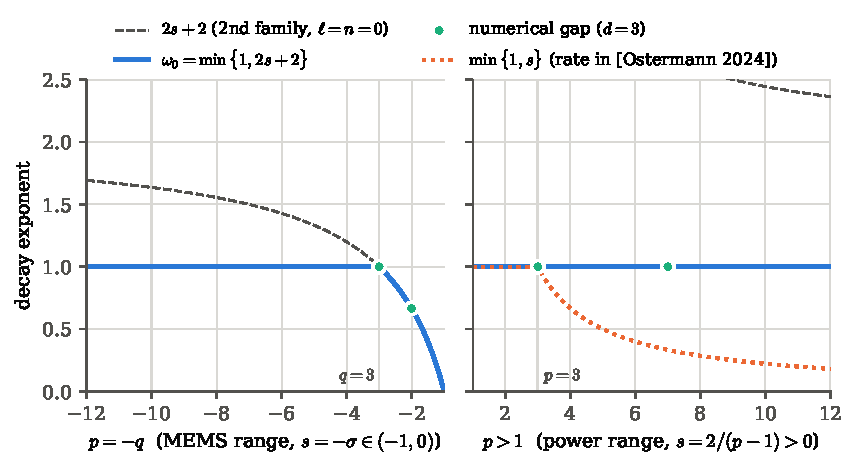
\includegraphics[width=0.92\textwidth]{figures/power_gap.pdf}
\caption{Spectral gap $\omega_0=\min\{1,2s+2\}$ over the MEMS range $p=-q<-1$
(left) and $p>1$ (right). Dashed: top of the second family, $2s+2$; dotted:
the exponent $\min\{1,s\}$ of \cite{Ostermann2024}, reflecting the free
eigenvalue $-s$; dots: numerically confirmed gaps ($d=3$).}
\label{power:fig-gap}
\end{figure}

\subsection{Summary and caveats}
\label{power:subsec-summary}

\textbf{(P)}: for all $p\notin[-1,1]$ (powers and MEMS), $V_0=(s+1)(s+2)$; the
spectrum in $\operatorname{Re}\lambda>-\omega_k$, $\omega_k=k-s_c$, is
$\{1-\ell-2n\}\cup\{-2s-2-\ell-2n\}$ with polynomial eigenfunctions; $\lambda=1$ and
the $d$-fold $\lambda=0$ are semisimple symmetry modes; the gap is
$\min\{1,2s+2\}$ ($=\frac23$ for $q=2$); Jordan blocks at $s=\pm\frac12$; no
self-similar ODE blowup for $-1\le p\le1$; the tilted family survives damping.
\textbf{(S)}: the free-flow splitting, the improved rate $1-\varepsilon$ for $p>1$,
\cref{power:lem-lower-order} and \cref{power:thm-lower-order}, conditional on the
autonomous linear estimate (for MEMS, \cref{mems:sec}). \textbf{(N)}: the
monodromy confirmation; Jordan blocks at all collisions; the co-dimension
claims of \cite{BizonMaisonWasserman2007}. Caveats: exponential decay needs
$k>s_c$ but the nonlinear argument uses $k>\frac d2$; the models are only valid up
to amplitudes where the cubic foundation law (or parallel-plate force) holds;
the literature in \cref{power:subsec-lit} was checked against abstracts, not
full texts.
